\chapter{Klassendokumentation}

\section{Service}

\subsection{TruffleReceiver}

\begin{figure}[h!]
    \centering
    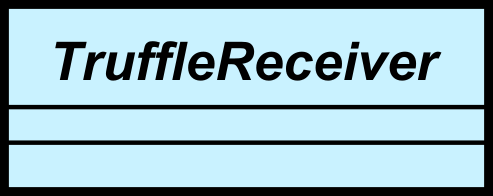
\includegraphics[width=\textwidth]{../diagramimages/TruffleReceiver.png}
    \caption[Klasse TruffleReceiver]{Klasse TruffleReceiver}
    \medskip
    Diese Klasse empfängt ganz tolle Truffles und so ein zeug bla bla.
\end{figure}

\subsubsection*{Attribute}

\begin{easylist}[itemize]

    & Attribut 1

    & Attribut 2

\end{easylist}

\subsubsection*{Methoden}

\begin{easylist}[itemize]

    & Methode 1

    & Methode 2

\end{easylist} 